\documentclass[12pt,a4paper,oneside]{report}

\usepackage[utf8]{inputenc}
\usepackage[T1]{fontenc}
\IfFileExists{lmodern.sty}{\usepackage{lmodern}}{}
\usepackage[margin=2.5cm]{geometry}
\usepackage{amsmath,amssymb,amsfonts,bm,mathtools}
\usepackage{graphicx}
\usepackage{booktabs}
\usepackage{multirow}
\usepackage{array}
\usepackage{xcolor}
\usepackage{tikz}
\usetikzlibrary{arrows.meta,positioning,fit,calc}
\usepackage[numbers,sort&compress]{natbib}
\usepackage{setspace}
\usepackage{caption}
\usepackage{subcaption}
\usepackage[hidelinks]{hyperref}

\onehalfspacing
\graphicspath{{figures/}}

% ---- notation
\newcommand{\R}{\mathbb{R}}
\newcommand{\C}{\mathbb{C}}
\newcommand{\vect}[1]{\bm{#1}}
\newcommand{\mat}[1]{\mathbf{#1}}
\newcommand{\norm}[1]{\left\lVert #1 \right\rVert}
\newcommand{\todo}[1]{\textcolor{red}{[#1]}}

% ---- fill in
\newcommand{\thesistitle}{Gaussian Splatting for Physical Inverse Problems:\\[0.3em]
  3D Gaussians for Inverse Scattering and 4D Gaussians for Fluid Dynamics}
\newcommand{\authorname}{Muhammad Hussain Qureshi}
\newcommand{\rollno}{\todo{Roll number, e.g.\ MSxx26xxx}}
\newcommand{\advisorname}{\todo{Advisor name}}
\newcommand{\department}{Faculty of Sciences}
\newcommand{\university}{Information Technology University (ITU), Lahore}
\newcommand{\submissiondate}{December 2026}

\begin{document}

% ================================================================ title page
\begin{titlepage}
  \centering
  \vspace*{1.5cm}
  {\LARGE\bfseries \thesistitle\par}
  \vspace{1.5cm}
  {\large Thesis I Report\par}
  \vspace{1.5cm}
  {\large \authorname\par}
  {\large \rollno\par}
  \vspace{1.0cm}
  {\large Advisor: \advisorname\par}
  \vfill
  {\large \department\\ \university\par}
  \vspace{0.5cm}
  {\large \submissiondate\par}
\end{titlepage}

\pagenumbering{roman}

\chapter*{Abstract}
\addcontentsline{toc}{chapter}{Abstract}
3D Gaussian Splatting represents a scene as a set of anisotropic Gaussians and has become a leading
representation for photographic novel-view synthesis; its dynamic extension, 4D Gaussian Splatting, adds a
deformation network over time. Both are designed for posed RGB images. This thesis asks whether the same
representation is useful for \emph{scientific inverse problems}, where an unknown physical field must be recovered
from indirect, incomplete and noisy measurements produced by a known physics model. Using datasets and forward
models from the InverseBench benchmark, we study two problems: (i) linear inverse scattering, where the permittivity
of cells is recovered from scattered electromagnetic fields measured by 360, 180 or 60 receivers, in 2D and on 3D
cell volumes; and (ii) the 2D incompressible Navier--Stokes equations, where an evolving vorticity field is
reconstructed from dense or sparse observations over time with a 4D (space--time) Gaussian representation whose
deformation is modelled either by a multilayer perceptron, as in 4D Gaussian Splatting, or by a Mamba selective
state-space model. We replace the camera rasteriser with the physics operator, render Gaussians on a grid with a
local-window evaluation, and train end-to-end by gradient descent with 3DGS-style densification and pruning.

The proof of concept shows that (1) on smooth 3D cell volumes, Gaussians are markedly more robust than a voxel
grid when measurements are scarce (40.9 vs.\ 37.3\,dB PSNR at 60 receivers), whereas on real sharp-edged nuclei
(BBBC024) and textured 2D cells the grid is better, so the benefit depends on the object matching the smooth Gaussian
prior; (2) adaptive densification can grow ``ghost'' copies of the object in regions the measurements cannot see
(the operator's null space), which a simple sparsity term removes; and (3) for fluid flow, a deformation model is
essential (+10\,dB over static Gaussians), and a Mamba deformation model with temporal smoothness generalises to
unobserved time steps better than the MLP of 4D Gaussian Splatting when only 10\% of pixels are observed
(25.4 vs.\ 23.0\,dB). These results establish feasibility and point to the open problems addressed in Thesis II.

\tableofcontents
\listoffigures
\listoftables

\clearpage
\pagenumbering{arabic}

\chapter{Introduction}
\label{ch:intro}

\section{Motivation}
Many measurements in science do not show the quantity of interest directly. An optical tomography system records how
light is scattered by a cell, not the cell's refractive index; a fluid experiment samples the flow at a few points and
times, not the full velocity or vorticity field. Recovering the hidden quantity from such indirect, incomplete and
noisy data is an \emph{inverse problem}. Inverse problems are typically ill-posed: many different unknowns explain
the measurements equally well, so the representation of the unknown and the prior knowledge built into it decide
which solution is found.

In computer vision, 3D Gaussian Splatting (3DGS)~\citep{kerbl20233dgs} has recently changed how scenes are
represented. Instead of a pixel or voxel grid, or a neural network evaluated at every point~\citep{mildenhall2020nerf},
a scene is a set of anisotropic Gaussians with learnable positions, shapes and amplitudes. The representation is
compact, adapts its resolution to the content through densification and pruning, and is differentiable, so it can be
fitted to measurements by gradient descent. Its dynamic extension, 4D Gaussian Splatting~\citep{wu20244dgs}, keeps
one canonical set of Gaussians and learns a deformation network that moves them over time.

Gaussians are also a natural basis for many physical fields: cell nuclei are smooth blobs, and vortices in a fluid are
localised, smooth structures that are carried along by the flow. This suggests that a Gaussian representation could
act as a useful structural prior for scientific inverse problems. Whether it does, and under which conditions, has not
been studied systematically: existing Gaussian methods for scientific imaging target specific modalities such as
X-ray computed tomography~\citep{cai2024xgaussian,zha2024r2gaussian}, while the recent InverseBench
benchmark~\citep{zheng2025inversebench} evaluates diffusion-model priors, not explicit Gaussian representations.

\section{Problem statement (summary)}
This thesis studies 3D and 4D Gaussian representations as the unknown in physics-based inverse problems. Given a
known forward model $\mathcal{A}$ that maps a physical field to measurements, and measurements
$\vect{y}=\mathcal{A}(f)+\vect{n}$, we represent $f$ by Gaussians and fit their parameters so that the simulated
measurements match $\vect{y}$. We ask when this representation helps compared with a plain grid of unknowns, how it
fails, and how its motion over time should be modelled. The full problem definition and scope are given in
Chapter~\ref{ch:problem}.

\section{Contributions of Thesis I}
\begin{enumerate}
  \item \textbf{Dataset analysis.} A study of the five InverseBench problems with respect to their suitability for
  3D and 4D Gaussian representations, leading to the choice of linear inverse scattering (3D) and Navier--Stokes (4D).
  \item \textbf{A physics-driven Gaussian pipeline.} A single implementation that renders 2D/3D Gaussians on a grid
  with a local-window evaluation, couples them to the InverseBench scattering operator (verified to match the
  benchmark implementation to within $3\times10^{-7}$ relative error) and to observations of the Navier--Stokes
  solution, and trains them with densification, pruning and an optional sparsity term.
  \item \textbf{4D Gaussians with a state-space motion model.} A 4D (2D + time) Gaussian representation whose
  deformation is modelled either by an MLP, as in 4D Gaussian Splatting, or by a Mamba selective state-space
  model~\citep{gu2023mamba} that treats each Gaussian's trajectory as a sequence.
  \item \textbf{Initial results and a failure analysis.} Baseline comparisons against pixel/voxel optimisation with
  identical physics, and the identification of a ``ghost'' failure mode caused by the operator's null space, with a
  sparsity-based remedy.
  \item \textbf{Open, reproducible code.} A public repository with a Python package, experiment configurations,
  notebooks, unit tests and all results so far (Appendix~\ref{app:repro}).
\end{enumerate}

\section{Outline}
Chapter~\ref{ch:background} introduces inverse problems, the two physical models and Gaussian splatting.
Chapter~\ref{ch:literature} reviews related work. Chapter~\ref{ch:problem} defines the problem, research questions
and scope. Chapter~\ref{ch:method} describes the pipeline and Chapter~\ref{ch:formulation} its mathematical
formulation. Chapter~\ref{ch:setup} gives the experimental setup and Chapter~\ref{ch:results} the initial results.
Chapter~\ref{ch:conclusion} discusses limitations and the plan for Thesis II.

\chapter{Background}
\label{ch:background}

\section{Inverse problems}
An inverse problem asks for an unknown $f$ from measurements
\begin{equation}
  \vect{y} = \mathcal{A}(f) + \vect{n},
\end{equation}
where $\mathcal{A}$ is a known forward model (here, a physics simulator) and $\vect{n}$ is noise. The problem is
\emph{ill-posed} when a solution does not exist, is not unique, or does not depend continuously on the data. In the
problems studied here there are far fewer measurements than unknowns, so $\mathcal{A}$ has a large null space: many
fields produce exactly the same measurements. A solution is therefore chosen by a prior, either explicit, as a
regularisation term such as total variation~\citep{rudin1992tv} or sparsity, or implicit, through the
\emph{parametrisation} of the unknown. A convolutional network trained on a single image acts as such an implicit
prior~\citep{ulyanov2018dip}; diffusion models trained on many examples act as a learned prior and are the subject of
InverseBench~\citep{zheng2025inversebench,chung2023dps}. In this thesis the prior is the Gaussian representation
itself, optionally combined with a sparsity term.

\section{Linear inverse scattering}
In optical diffraction tomography an object is illuminated by a known incident field and the scattered field is
recorded by receivers around it~\citep{bornwolf1999}. For a weakly scattering object the total field inside the object
can be approximated by the incident field (the first Born approximation), and the scattered field becomes a
\emph{linear} function of the object's permittivity contrast $f(\vect{x})$:
\begin{equation}
  u^{\mathrm{sc}}_t(\vect{r}) = k_b^2 \int_\Omega G(\vect{r},\vect{x})\, f(\vect{x})\, u^{\mathrm{in}}_t(\vect{x})\, d\vect{x},
  \qquad G(\vect{r},\vect{x}) = \tfrac{i}{4} H_0^{(1)}\!\left(k_b \lVert \vect{r}-\vect{x}\rVert\right),
\end{equation}
where $t$ indexes the transmitter, $\vect{r}$ a receiver position, $k_b$ the background wavenumber and $H_0^{(1)}$
the Hankel function of the first kind (the 2D Green's function). Multiple-scattering models drop the Born
approximation at a higher cost~\citep{sun2018multiplescattering}. InverseBench uses the linear model with 20
transmitters on a circle and 360, 180 or 60 receivers on the same circle, a $128\times128$ grid of a
$0.18\times0.18$\,m domain, and cell images simulated with CytoPacq~\citep{wiesner2019cytopacq}.

\section{Incompressible Navier--Stokes flow}
The 2D incompressible Navier--Stokes equations in vorticity form on the periodic domain $[0,2\pi]^2$ are
\begin{equation}
  \partial_t \omega + \vect{u}\cdot\nabla\omega = \frac{1}{Re}\,\Delta\omega + g, \qquad
  \vect{u} = (\partial_y\psi,\,-\partial_x\psi), \qquad -\Delta\psi = \omega,
\end{equation}
with vorticity $\omega$, velocity $\vect{u}$, stream function $\psi$, Reynolds number $Re$ and forcing $g$. Vorticity
is transported by the flow and diffused by viscosity, so its structures move and deform smoothly over time. InverseBench
uses $Re=200$, forcing $g=-4\cos(4y)$ and a pseudo-spectral solver; this problem is also a standard benchmark for
neural PDE solvers~\citep{li2021fno}.

\section{Neural fields and Gaussian splatting}
\paragraph{Neural radiance fields.} NeRF~\citep{mildenhall2020nerf} represents a scene by an MLP that maps a 3D
position and viewing direction to colour and density and renders images by volume rendering along camera rays. Fourier
features of the input coordinates allow MLPs to represent high frequencies~\citep{tancik2020fourier}. Grid- and
hash-based encodings make such fields much faster~\citep{mueller2022instantngp}.

\paragraph{3D Gaussian Splatting.} 3DGS~\citep{kerbl20233dgs} replaces the MLP by an explicit set of anisotropic 3D
Gaussians, each with a mean, a covariance factorised into a rotation and scales, an opacity and a colour. Gaussians are
projected (``splatted'') onto the image plane and alpha-blended; all parameters are optimised by gradient descent.
\emph{Adaptive density control} clones or splits Gaussians where reconstruction gradients are large and prunes
transparent ones, so the representation spends its capacity where the scene needs it.

\paragraph{Dynamic scenes.} D-NeRF~\citep{pumarola2021dnerf} introduced a canonical space plus a deformation network
for dynamic NeRFs. 4D Gaussian Splatting~\citep{wu20244dgs} applies the same idea to Gaussians, predicting per-time
offsets of position, scale and rotation from a spatio-temporal feature encoding (HexPlane~\citep{cao2023hexplane}).
Alternatives include per-frame Gaussians tracked over time~\citep{luiten2024dynamic} and native 4D
Gaussians~\citep{yang2024realtime4dgs}.

\section{State-space sequence models and Mamba}
Structured state-space models (S4)~\citep{gu2022s4} model sequences with a linear recurrence
$\vect{h}_t = \bar{\mat{A}}\vect{h}_{t-1} + \bar{\mat{B}}x_t$, $y_t = \mat{C}\vect{h}_t$, obtained by discretising a
continuous-time system. Mamba~\citep{gu2023mamba} makes the step size $\Delta$ and the matrices $\mat{B}$, $\mat{C}$
functions of the input (\emph{selection}), so the model can decide what to keep in its state, and computes the
recurrence with a hardware-efficient scan in time linear in the sequence length. Mamba has been applied to vision
backbones~\citep{zhu2024visionmamba}. Here it is used to model how each Gaussian moves through time.

\chapter{Literature Review}
\label{ch:literature}

This chapter reviews four lines of work that meet in this thesis: (1) learned priors for scientific inverse problems,
(2) explicit Gaussian representations, (3) Gaussian and neural-field methods for scientific and medical imaging, and
(4) dynamic representations and sequence models. It closes with the gap this thesis addresses.

\section{Priors for scientific inverse problems}
Classical solvers combine a data-fidelity term with hand-crafted regularisers such as total
variation~\citep{rudin1992tv}. Deep learning added two families of priors. \emph{Untrained} priors use the structure
of a network as the regulariser: Deep Image Prior~\citep{ulyanov2018dip} fits a randomly initialised convolutional
network to a single corrupted image and stops early. \emph{Learned} priors are trained on many examples; diffusion
models are currently the most general, and Diffusion Posterior Sampling~\citep{chung2023dps} guides the reverse
diffusion with the gradient of the data likelihood, so the same prior can serve many forward models.

InverseBench~\citep{zheng2025inversebench} evaluates 14 such plug-and-play diffusion-prior algorithms on five
scientific problems: linear inverse scattering, compressed-sensing MRI on fastMRI~\citep{zbontar2018fastmri}, black
hole imaging, full waveform inversion on OpenFWI~\citep{deng2022openfwi}, and the 2D Navier--Stokes equations. Its
findings that motivate this thesis are that (i) scientific forward models differ strongly from image-restoration
operators (complex-valued, non-linear, expensive, or without gradients), (ii) diffusion priors help most when
measurements are sparse, and (iii) they can fail when outputs violate physical constraints. All its methods represent
the unknown on a pixel grid. Physics-informed neural networks~\citep{raissi2019pinn} and neural operators such as
FNO~\citep{li2021fno} are complementary: they learn solution operators of PDEs rather than priors over unknowns.

\section{Explicit Gaussian representations}
3DGS~\citep{kerbl20233dgs} showed that an explicit, adaptive set of anisotropic Gaussians can match or exceed neural
fields~\citep{mildenhall2020nerf,mueller2022instantngp} in quality while rendering in real time. Its key ingredients
are a differentiable rasteriser, a covariance parametrisation by rotation and scale that stays positive
semi-definite, and adaptive density control. GaussianImage~\citep{zhang2024gaussianimage} transfers the idea to 2D:
an image is represented by 2D Gaussians and rendered by accumulated summation, achieving fast decoding and
compression. Our 2D and 3D representations follow the same principle, but are evaluated on a regular grid and
supervised through a physics operator instead of pixels.

\section{Gaussians and neural fields in scientific imaging}
\paragraph{Tomography.} X-Gaussian~\citep{cai2024xgaussian} adapts Gaussian splatting to X-ray projection imaging
with a radiative Gaussian model, and R$^2$-Gaussian~\citep{zha2024r2gaussian} rectifies the integration bias of
splatting for tomographic volume reconstruction, showing that Gaussians can serve as a voxel-free representation of
attenuation volumes. Both rely on ray-based projection, the natural analogue of camera rendering; scattering
measurements are instead a wave-based integral over the whole object.
\paragraph{Astronomy.} BH-NeRF~\citep{levis2022bhnerf} reconstructs 3D emission around a black hole over time with a
neural field constrained by gravitational lensing and orbital dynamics, an example of physics replacing multi-view
geometry.
\paragraph{Microscopy data.} Simulated cell images with exact ground truth are produced by CytoPacq and related
generators~\citep{wiesner2019cytopacq}; the Broad Bioimage Benchmark Collection~\citep{ljosa2012bbbc} distributes such
synthetic 3D nucleus datasets (BBBC024), which we use as real 3D cell shapes.

\section{Dynamic representations and sequence models}
D-NeRF~\citep{pumarola2021dnerf} and 4D Gaussian Splatting~\citep{wu20244dgs} model motion with a canonical
representation and a deformation field queried independently at each time; HexPlane~\citep{cao2023hexplane} and
K-Planes~\citep{fridovich2023kplanes} factorise space--time features into planes. Dynamic 3D
Gaussians~\citep{luiten2024dynamic} track persistent Gaussians frame by frame, and native 4D
Gaussians~\citep{yang2024realtime4dgs} slice 4D primitives in time. Language-embedded variants
(LangSplat~\citep{qin2024langsplat}, 4D LangSplat~\citep{li2025langsplat4d}) attach semantic features to such
Gaussians, the starting point of this thesis' original direction. None of these treats a Gaussian's trajectory as a
sequence. State-space models~\citep{gu2022s4,gu2023mamba} are efficient sequence models that could do exactly that,
and have been adopted in vision~\citep{zhu2024visionmamba}; their use as a motion model for 4D Gaussians is, to our
knowledge, unexplored.

\section{Synthesis and research gap}
Table~\ref{tab:lit} summarises the landscape. Diffusion-prior methods are general but represent the unknown on a
grid and need large training sets; Gaussian methods are compact and adaptive but have been demonstrated mainly with
camera- or ray-based measurements. The gap addressed here is the use of 3D/4D Gaussian representations as the unknown
in \emph{wave-based and PDE-based scientific inverse problems}, the analysis of their failure modes under severe
ill-posedness, and sequence-model motion priors for their dynamics.

\begin{table}[t]
  \centering
  \small
  \caption{Representative related work. ``Meas.'' is the kind of measurement used for supervision.}
  \label{tab:lit}
  \begin{tabular}{p{3.6cm}p{2.6cm}p{2.7cm}p{4.6cm}}
    \toprule
    Work & Representation & Meas. & Relation to this thesis \\
    \midrule
    NeRF~\citep{mildenhall2020nerf} & MLP field & RGB images & implicit field; rendering by rays \\
    3DGS~\citep{kerbl20233dgs} & 3D Gaussians & RGB images & our representation, without cameras \\
    4DGS~\citep{wu20244dgs} & Gaussians + deformation & video & our 4D design (MLP deformation) \\
    GaussianImage~\citep{zhang2024gaussianimage} & 2D Gaussians & pixels & 2D Gaussian rendering on a grid \\
    X-Gaussian~\citep{cai2024xgaussian}, R$^2$-Gaussian~\citep{zha2024r2gaussian} & 3D Gaussians & X-ray projections & Gaussians for physics, ray-based \\
    BH-NeRF~\citep{levis2022bhnerf} & neural field & radio interferometry & physics replaces multi-view geometry \\
    DPS~\citep{chung2023dps}, InverseBench~\citep{zheng2025inversebench} & pixel grid + diffusion prior & physics operators & same problems, learned prior \\
    Mamba~\citep{gu2023mamba} & selective SSM & sequences & our motion model over time \\
    \textbf{This thesis} & 2D/3D/4D Gaussians & scattering; sparse flow samples & Gaussians + physics; Mamba motion \\
    \bottomrule
  \end{tabular}
\end{table}

\chapter{Problem Definition and Research Scope}
\label{ch:problem}

\section{Problem definition}
Let $f:\Omega\to\R$ be an unknown physical field on a domain $\Omega\subset\R^d$ (permittivity contrast of a cell,
$d\in\{2,3\}$), or a time-dependent field $\omega:\Omega\times[0,T]\to\R$ (vorticity of a flow, $d=2$). A known forward
model $\mathcal{A}$ produces measurements $\vect{y}=\mathcal{A}(f)+\vect{n}$ with
$\dim\vect{y}\ll\dim f$. We represent the unknown by a set of $N$ Gaussians with parameters
$\Theta=\{\theta_i\}_{i=1}^N$ (and, for dynamic fields, a deformation network with weights $\phi$) and solve
\begin{equation}
  \hat\Theta = \arg\min_{\Theta}\; \mathcal{D}\big(\mathcal{A}(f_\Theta),\vect{y}\big) + \mathcal{R}(\Theta),
\end{equation}
where $\mathcal{D}$ measures data misfit and $\mathcal{R}$ is an optional regulariser. The ground truth is never used
for fitting; it is used only to evaluate the reconstruction.

\section{Research questions}
\begin{description}
  \item[RQ1] Can 2D/3D Gaussian representations recover physical fields from scattering measurements, and how do they
  compare with a pixel/voxel grid optimised with the same physics as the number of measurements decreases?
  \item[RQ2] What failure modes arise when an adaptive Gaussian representation meets an operator with a large null
  space, and how can they be prevented?
  \item[RQ3] Can a 4D Gaussian representation (canonical Gaussians plus deformation) reconstruct an evolving fluid
  field from dense and sparse observations, including at time steps that were never observed?
  \item[RQ4] Does a selective state-space model (Mamba) over each Gaussian's trajectory model the dynamics better than
  the per-time MLP deformation of 4D Gaussian Splatting?
\end{description}

\section{Scope}
\paragraph{In scope (Thesis I).}
\begin{itemize}
  \item Linear inverse scattering with the InverseBench forward model: 2D cells (InverseBench test set) and 3D cell
  volumes (synthetic HL60-like nuclei and CytoPacq/BBBC024 nuclei), with 360, 180 and 60 receivers and the benchmark
  noise level.
  \item 3D physics with two models: the 2D operator applied to every $z$-slice (\emph{slice-wise}) and a \emph{true 3D}
  first-order Born model with transmitters and receivers on a sphere around the volume.
  \item 2D Navier--Stokes ($Re=200$) as a 2D + time (``4D'') problem: sequences of 21 frames, observations of all or
  10\% of the pixels per frame, every fourth frame held out.
  \item Baselines: direct optimisation of a pixel/voxel grid with the same data term (and the same sparsity term).
  \item Metrics: PSNR, SSIM, relative $\ell_2$ error, number of Gaussians, run time.
\end{itemize}
\paragraph{Out of scope (deferred to Thesis II).}
\begin{itemize}
  \item A full 3D scattering model with sensors on a sphere, and non-linear (multiple-scattering) physics.
  \item Recovering the Navier--Stokes \emph{initial condition} through the solver, as posed in InverseBench.
  \item Exhaustive benchmarking against the diffusion-prior methods of InverseBench; training learned priors.
  \item Real (non-simulated) measurement data, and the remaining InverseBench problems.
\end{itemize}

\section{Assumptions}
The forward models are known exactly and are differentiable; measurement noise is additive Gaussian at the benchmark
level ($\sigma=10^{-4}$ for scattering); permittivity contrast is non-negative and bounded in $[0,1]$; vorticity is
periodic in space.

\chapter{Proposed Methodology and Pipeline Architecture}
\label{ch:method}

\section{Overview}
The same training loop serves every task (Figure~\ref{fig:pipeline}). A set of Gaussians is rendered on the grid of
the unknown; a physics operator turns the rendered field into simulated measurements; the misfit to the real
measurements, plus an optional sparsity term, is back-propagated to all Gaussian parameters; and an adaptive density
control step periodically adds and removes Gaussians. For dynamic fields a deformation network maps the canonical
Gaussians to their state at each time step before rendering.

\begin{figure}[t]
\centering
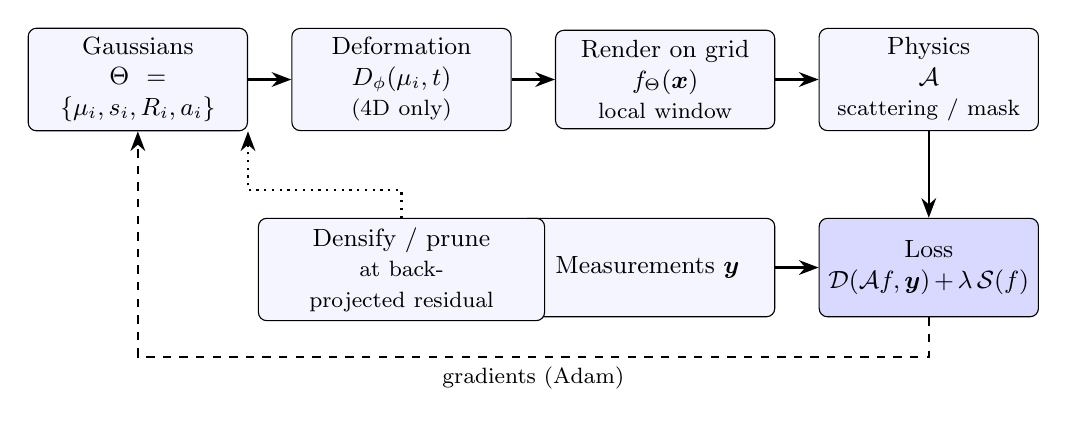
\begin{tikzpicture}[
  box/.style={draw, rounded corners=3pt, align=center, minimum height=1.25cm, text width=2.55cm, font=\small, fill=blue!4},
  dark/.style={box, fill=blue!15},
  arr/.style={-{Stealth[length=2.5mm]}, thick},
  node distance=0.55cm]
  \node[box] (g) {Gaussians\\$\Theta=\{\mu_i,s_i,R_i,a_i\}$};
  \node[box, right=of g] (d) {Deformation\\$D_\phi(\mu_i,t)$\\{\footnotesize (4D only)}};
  \node[box, right=of d] (r) {Render on grid\\$f_\Theta(\vect{x})$\\{\footnotesize local window}};
  \node[box, right=of r] (a) {Physics\\$\mathcal{A}$\\{\footnotesize scattering / mask}};
  \node[dark, below=1.1cm of a] (l) {Loss\\$\mathcal{D}(\mathcal{A}f,\vect{y})+\lambda\,\mathcal{S}(f)$};
  \node[box, left=of l, text width=3.0cm] (y) {Measurements $\vect{y}$};
  \node[box, below=1.1cm of d, text width=3.4cm] (dc) {Densify / prune\\{\footnotesize at back-projected residual}};
  \draw[arr] (g) -- (d); \draw[arr] (d) -- (r); \draw[arr] (r) -- (a); \draw[arr] (a) -- (l); \draw[arr] (y) -- (l);
  \draw[arr, dashed] (l.south) -- ++(0,-0.5) -| node[pos=0.25, below, font=\footnotesize]{gradients (Adam)} (g.south);
  \draw[arr, dotted] (dc.north) -- ++(0,0.35) -| (g.south east);
\end{tikzpicture}
\caption{Pipeline. The camera rasteriser of 3DGS is replaced by rendering on a grid followed by the physics operator.}
\label{fig:pipeline}
\end{figure}

\section{Gaussian field representation}
Each Gaussian has a centre, per-axis scales, an orientation and an amplitude; the field at a grid point is the sum of
all Gaussians evaluated there (Section~\ref{sec:field}). Because a Gaussian is negligible beyond about three standard
deviations, each Gaussian is evaluated only in a window of $\pm h$ cells around its centre and accumulated into the
grid with a scatter-add, so the cost is $O(N(2h+1)^d)$ and independent of the grid size; scales are clamped to
$h/3$ so that the window always covers $\pm3\sigma$. For permittivity the amplitude is kept non-negative with a
softplus; for vorticity it is signed and the window wraps around the periodic domain. All parameters of one scene form
a single $N\times P$ tensor ($P=6$ in 2D, $P=11$ in 3D), which is convenient for sequence models.

\section{Physics operators}
\paragraph{Scattering.} We re-implement the InverseBench linear scattering operator as two complex matrix products
in single precision on the GPU and verify at start-up that it matches the benchmark implementation to within a relative
error of $3\times10^{-7}$. For 3D volumes, the operator is applied to every $z$-slice and the losses are summed.
\paragraph{Fluid observations.} For Navier--Stokes the measurement operator selects the observed pixels of each frame
(a random mask with 100\% or 10\% coverage); frames that are held out for evaluation are never observed.

\section{Training and adaptive density control}
All parameters are optimised with Adam~\citep{kingma2015adam} and a cosine learning-rate schedule. For scattering,
Gaussians are initialised uniformly at random, with no knowledge of the object. Every 250 iterations, during the
first 60\% of training, new Gaussians are inserted at the grid points with the largest magnitude of the
\emph{back-projected residual} $\mathrm{Re}\,\mathcal{A}^{\mathsf H}(\vect{y}-\mathcal{A}f)$, i.e.\ where the
measurements indicate missing structure, and Gaussians whose amplitude has fallen below $10^{-3}$ are pruned. This
replaces the image-space gradient criterion of 3DGS, which is unavailable without pixel supervision.

\section{Sparsity regulariser}
Early experiments showed that aggressive densification can place mass in regions to which the measurements are blind
(Section~\ref{sec:ghost}). A sparsity term on the total intensity of the rendered field penalises mass the data does
not require. Because the field is non-negative, the mean of the field equals its $\ell_1$ norm divided by the grid size.

\section{4D representation of fluid flow}
A canonical set of 2D Gaussians is initialised from the observed pixels of the first frame. A deformation network maps
each Gaussian's canonical centre and the time $t$ to offsets of all its parameters; positions move in pixel units.
Three deformation models are compared:
\begin{itemize}
  \item \textbf{MLP} (as in 4D Gaussian Splatting): Fourier features of $(\mu_i,t)$ fed to a three-layer MLP,
  evaluated independently for every Gaussian and time.
  \item \textbf{Mamba}: for each Gaussian the inputs at all $T$ time steps form a sequence processed by two Mamba
  blocks, so the offset at time $t$ depends on the Gaussian's earlier states (causal).
  \item \textbf{Bidirectional Mamba}: a second Mamba stack reads the sequence backwards and the two are summed, so
  every time step sees both past and future.
\end{itemize}
The output layer is initialised to zero so training starts from the canonical configuration. An optional temporal
smoothness term penalises differences between offsets at consecutive times, including unobserved times. A
\emph{static} model without deformation serves as an ablation.

\section{Baselines}
The baseline for scattering optimises every pixel (2D) or voxel (3D) directly with the same data term, starting from
zero and projected to $[0,1]$ after each step; optionally it uses the same sparsity term. Only the representation
differs between the two methods. For fluids, the static-Gaussian model is the baseline.

\section{Implementation}
The pipeline is a Python/PyTorch package (\texttt{thesis\_gs}) with modules for the Gaussian field, physics,
volume loading, scattering experiments, Navier--Stokes data, deformation networks and 4D training, a command-line
interface, experiment configurations and unit tests (Appendix~\ref{app:repro}). Mamba is implemented in pure PyTorch
with an explicit selective scan, which is sufficient for sequences of 21 steps and runs on any GPU.

\chapter{Mathematical Formulation}
\label{ch:formulation}

\section{Gaussian field}
\label{sec:field}
A field on a grid with points $\vect{x}\in\Omega\subset\R^d$ is represented by $N$ Gaussians,
\begin{equation}
  f_\Theta(\vect{x}) = \sum_{i=1}^{N} a_i \exp\!\Big(-\tfrac12(\vect{x}-\vect{\mu}_i)^\top \mat{\Sigma}_i^{-1}(\vect{x}-\vect{\mu}_i)\Big),
  \qquad \mat{\Sigma}_i = \mat{R}_i\,\mathrm{diag}(\vect{s}_i)^2\,\mat{R}_i^\top ,
  \label{eq:field}
\end{equation}
with centre $\vect{\mu}_i\in\R^d$, scales $\vect{s}_i=\exp(\vect{\ell}_i)$ clamped to $[s_{\min},h/3]$, and rotation
$\mat{R}_i$: in 2D $\mat{R}(\vartheta_i)=\begin{psmallmatrix}\cos\vartheta_i & -\sin\vartheta_i\\ \sin\vartheta_i & \cos\vartheta_i\end{psmallmatrix}$,
in 3D the rotation matrix of the normalised quaternion $\vect{q}_i/\lVert\vect{q}_i\rVert$. The factorisation keeps
$\mat{\Sigma}_i$ symmetric positive definite for any parameter values~\citep{kerbl20233dgs}. The amplitude is
$a_i=\mathrm{softplus}(\alpha_i)\ge0$ for permittivity and $a_i=\alpha_i\in\R$ for vorticity. The parameters per
Gaussian are $\theta_i=(\vect{\mu}_i,\vect{\ell}_i,\vartheta_i\text{ or }\vect{q}_i,\alpha_i)$. In practice the sum in
\eqref{eq:field} runs only over Gaussians whose window $\lVert\vect{x}-\mathrm{round}(\vect{\mu}_i)\rVert_\infty\le h$
contains $\vect{x}$. A \emph{generalised} Gaussian replaces the quadratic form $q_i(\vect{x})$ in the exponent by
$q_i(\vect{x})^{\beta}$ with $\beta\ge1$: $\beta=1$ is \eqref{eq:field}, larger $\beta$ gives a flatter top and a sharper
edge, intended for piecewise-constant objects.

\paragraph{Bounded density.} The sum \eqref{eq:field} is unbounded: overlapping Gaussians can exceed the physical
range of the contrast, whereas the grid baseline is projected onto $[0,1]$ after every step. The bounded variant
renders
\begin{equation}
  \tilde f_\Theta(\vect{x}) = 1-\exp\!\big(-f_\Theta(\vect{x})\big)\in[0,1),
  \label{eq:bounded}
\end{equation}
the same saturation as opacity accumulation in 3DGS. It is smooth, monotone and close to $f_\Theta$ for small values,
so it changes only where Gaussians overlap. Optionally the Gaussians are \emph{initialised from the grid solution}:
centres are sampled in proportion to $-\log(1-\min(f_{\text{grid}},0.95))$, the density that \eqref{eq:bounded} maps
back to the grid reconstruction, and then refined with the same physics loss.

\section{Scattering forward model}
On a grid of $P$ points with spacing $\Delta x\,\Delta y$, the linear (Born) scattering operator of the benchmark maps
a contrast image $\vect{f}\in\R^P$ to measurements for $T$ transmitters and $M$ receivers,
\begin{equation}
  y_{t,r} = \Delta x\,\Delta y \sum_{p=1}^{P} f_p\,\overline{u^{\mathrm{in}}_t(\vect{x}_p)}\,g_r(\vect{x}_p),
  \qquad g_r(\vect{x}) = k_b^2\,\tfrac{i}{4}H_0^{(1)}\!\big(k_b\lVert\vect{r}_r-\vect{x}\rVert\big),
  \label{eq:born}
\end{equation}
written compactly as $\vect{y}=\mat{A}\vect{f}+\vect{n}$ with $\mat{A}\in\C^{TM\times P}$ and complex Gaussian noise of
standard deviation $\sigma=10^{-4}$. Here $T=20$, $M\in\{360,180,60\}$ and $P=128^2$, so $TM\le7200$ complex
measurements describe $16384$ unknowns and $\mat{A}$ has a non-trivial null space. For a volume with slices
$\vect{f}^{(z)}$, $z=1,\dots,Z$, the slice-wise model is $\vect{y}^{(z)}=\mat{A}\vect{f}^{(z)}+\vect{n}^{(z)}$.

\paragraph{True 3D Born model.} The slice-wise model treats each slice as an independent 2D experiment. A true 3D
first-order Born model with point transmitters at $\vect{s}_t$ and receivers at $\vect{r}_r$ on a sphere around the
volume is
\begin{equation}
  y_{t,r} = k^2\,\Delta V \sum_{p=1}^{P} f_p\, G(\lVert\vect{s}_t-\vect{x}_p\rVert)\, G(\lVert\vect{r}_r-\vect{x}_p\rVert),
  \qquad G(d)=\frac{e^{\mathrm{i}kd}}{4\pi d},
  \label{eq:born3d}
\end{equation}
with the free-space Green's function of the 3D Helmholtz equation, voxel volume $\Delta V=\Delta x^3$ and the same
voxel size, wavelength (six voxels) and sensor radius (1.6\,m) as the 2D benchmark. We use $T=60$ transmitters and
$M\in\{360,180,60\}$ receivers spread evenly over the sphere (golden-angle spiral). A $32\times128\times128$ volume has
$P=524{,}288$ unknowns but only $TM\le21{,}600$ complex measurements, about a tenth of the slice-wise model, so the
problem is far more under-determined. Noise is complex Gaussian with standard deviation 2\% of the RMS measurement,
the signal-to-noise ratio of the 2D benchmark. The implementation matches the analytic response of a point scatterer
to $10^{-7}$ and passes an adjoint test $\langle\mat{A}\vect{f},\vect{r}\rangle=\langle\vect{f},\mat{A}^H\vect{r}\rangle$.

\section{Objective for scattering}
With $\vect{f}_\Theta$ the field \eqref{eq:field} sampled on the grid,
\begin{equation}
  \mathcal{L}(\Theta) = \frac{\sum_z \norm{\mat{A}\vect{f}^{(z)}_\Theta-\vect{y}^{(z)}}_2^2}{\sum_z\norm{\vect{y}^{(z)}}_2^2}
  \;+\; \lambda\,\frac{1}{|\Omega|}\sum_{\vect{x}\in\Omega} f_\Theta(\vect{x}),
  \label{eq:loss}
\end{equation}
where the second term equals $\lambda\norm{\vect{f}_\Theta}_1/|\Omega|$ because $f_\Theta\ge0$. The baseline solves
the same problem over the grid values directly,
$\min_{\vect{f}\in[0,1]^{|\Omega|}} \norm{\mat{A}\vect{f}-\vect{y}}_2^2/\norm{\vect{y}}_2^2+\lambda\,\overline{\vect{f}}$,
by projected Adam from $\vect{f}=\vect{0}$.

\paragraph{Why grids do not grow ghosts.} The gradient of the data term with respect to $\vect{f}$ is
$2\,\mathrm{Re}\,\mat{A}^{\mathsf H}(\mat{A}\vect{f}-\vect{y})/\norm{\vect{y}}^2$, which lies in the range of
$\mat{A}^{\mathsf H}$, the orthogonal complement of the null space. Gradient steps from zero therefore never add
null-space components (up to the effect of the projection onto $[0,1]$). Gaussians break this property: a Gaussian
inserted anywhere carries mass that may lie largely in the null space, where the data term exerts no force to remove it.
The sparsity term in \eqref{eq:loss} supplies that force.

\section{Adaptive density control}
Every $K=250$ iterations while $k\le0.6\,K_{\max}$ the back-projected residual
\begin{equation}
  \vect{\rho} = \mathrm{Re}\big(\mat{A}^{\mathsf H}(\vect{y}-\mat{A}\vect{f}_\Theta)\big)
\end{equation}
is computed, $n_{\mathrm{add}}$ new Gaussians are created at the grid points with the largest $|\rho|$ (scale 1.5
cells, amplitude proportional to $|\rho|$), and Gaussians with $a_i<10^{-3}$ are removed.

\section{4D representation}
For a sequence $\omega_0,\dots,\omega_{T-1}$ observed through masks $\mat{M}_t$, canonical parameters $\theta_i$ are
deformed by a network $D_\phi$:
\begin{equation}
  \theta_i(t) = \theta_i + \mat{S}\,D_\phi\big(\gamma(\vect{\mu}_i/L),\,\gamma(t/T)\big),
  \qquad \gamma(p) = \big[\sin(2^k\pi p),\cos(2^k\pi p)\big]_{k=0}^{K-1},
\end{equation}
where $\mat{S}$ scales position offsets to pixels and $\gamma$ are Fourier features~\citep{tancik2020fourier}. The
training loss over a random batch $\mathcal{B}$ of observed frames is
\begin{equation}
  \mathcal{L}(\Theta,\phi) = \sum_{t\in\mathcal{B}}
    \frac{\norm{\mat{M}_t\odot(f_{\Theta(t)}-\tilde\omega_t)}_2^2}{\norm{\mat{M}_t}_1}
  \;+\; \lambda_T \sum_{t\in\mathcal{B}}\frac{1}{N}\sum_i \norm{D_\phi(\cdot,t+1)-D_\phi(\cdot,t)}_2^2 ,
\end{equation}
with $\tilde\omega_t$ the (normalised) observations and $\lambda_T\ge0$ the temporal smoothness weight.

\section{Mamba deformation}
For Gaussian $i$, the inputs $\vect{x}_t$ ($t=0,\dots,T-1$) are linear embeddings of $[\gamma(\vect{\mu}_i),\gamma(t)]$.
A Mamba block~\citep{gu2023mamba} computes, after a gated input projection and a short causal convolution,
\begin{align}
  \Delta_t &= \mathrm{softplus}(\mat{W}_\Delta \vect{x}_t), \qquad \mat{B}_t = \mat{W}_B\vect{x}_t, \qquad \mat{C}_t = \mat{W}_C\vect{x}_t,\\
  \vect{h}_t &= \exp(\Delta_t\mat{A})\odot\vect{h}_{t-1} + \Delta_t\,\mat{B}_t\,\vect{x}_t, \qquad
  \vect{y}_t = \mat{C}_t\vect{h}_t + \mat{D}\vect{x}_t,
\end{align}
with a diagonal state matrix $\mat{A}=-\exp(\mat{A}_{\log})$, followed by multiplicative gating with
$\mathrm{SiLU}(\vect{z}_t)$ and a residual connection. Because $\Delta_t,\mat{B}_t,\mat{C}_t$ depend on the input, the
model selects what to remember along the trajectory. The bidirectional variant adds a second stack applied to the
time-reversed sequence and sums the two outputs.

\section{Evaluation metrics}
For a reconstruction $\hat f$ and ground truth $f$ with data range $R$,
\begin{equation}
  \mathrm{PSNR} = 10\log_{10}\frac{R^2}{\frac{1}{|\Omega|}\norm{\hat f-f}_2^2}, \qquad
  \mathrm{relL2} = \frac{\norm{\hat f-f}_2}{\norm{f}_2},
\end{equation}
and SSIM~\citep{wang2004ssim} computed with the default $7\times7$ uniform window of scikit-image ($R=1$ for permittivity,
$R=2$ for normalised vorticity). For 4D, metrics are averaged separately over observed (training) and held-out frames.

\chapter{Experimental Setup}
\label{ch:setup}

\section{Data}
\begin{itemize}
  \item \textbf{2D cells (scattering).} The first samples of the InverseBench \texttt{inv-scatter-test} set:
  $128\times128$ permittivity images of 1--6 HL60 nuclei simulated with CytoPacq~\citep{wiesner2019cytopacq}, values in
  $[0,1]$.
  \item \textbf{3D cells (scattering).} (a) Synthetic HL60-like nuclei generated by our code: 1--6 soft, rotated
  ellipsoids with smooth internal texture in a $32\times128\times128$ volume. (b) Real CytoPacq nuclei from BBBC024
  of the Broad Bioimage Benchmark Collection~\citep{ljosa2012bbbc} (ground-truth label masks, 20 nuclei per volume),
  converted to foreground masks, cropped to the central half in $x$ and $y$ and resampled to
  $32\times128\times128$.
  \item \textbf{Fluid (4D).} Initial vorticity fields from the InverseBench \texttt{navier-stokes-test} set
  ($Re=200$), rolled forward with the InverseBench pseudo-spectral solver to 21 frames spaced $\Delta t=0.05$
  apart, divided by 10 to lie in about $[-1,1]$. Frames 2, 6, 10, 14 and 18 are held out; the rest are observed
  completely or at a random 10\% of pixels per frame.
\end{itemize}

\section{Forward models and noise}
Scattering uses the InverseBench configuration: domain $0.18\times0.18$\,m, wavelength six grid cells, 20
transmitters and 360, 180 or 60 receivers on a circle of radius 1.6\,m, complex Gaussian noise $\sigma=10^{-4}$ with a
fixed seed per sample so that Gaussian and baseline fits see identical measurements.

\section{Hyper-parameters}
\begin{table}[h]
  \centering\small
  \caption{Default settings (overridable from the command line; every run stores its exact settings).}
  \label{tab:hparams}
  \resizebox{\linewidth}{!}{%
\begin{tabular}{lll}
    \toprule
    Setting & Scattering 2D / 3D & Fluid 4D \\
    \midrule
    Iterations & 3000 & 3000 \\
    Optimiser, learning rate & Adam, 0.05 (Gaussians), 0.01 (grid) & Adam, 0.01 (Gaussians), $10^{-3}$ (network) \\
    Schedule & cosine & cosine \\
    Max.\ / initial Gaussians & 2000 / 250 (2D); 8000 / 2000 (3D) & 2000 / 2000 \\
    Window half-size $h$ & 8 (2D), 6 (3D) & 10, periodic \\
    Densification & every 250 it., until 60\%, $+n_{\mathrm{init}}/4$ & none \\
    Sparsity $\lambda$ & 0, 0.1, 0.3, 1, 3 & -- \\
    Temporal smoothness $\lambda_T$ & -- & 0 (initial), 1 (final) \\
    Deformation & -- & MLP (3$\times$128), Mamba and bidirectional Mamba (2 blocks, $d=64$, state 16) \\
    Batch & one sample & 4 frames \\
    Samples per setting & 3 (5 in the final 2D runs) & 3 sequences \\
    \bottomrule
  \end{tabular}}
\end{table}

\section{Hardware and software}
All experiments ran on a single NVIDIA Tesla T4 (16\,GB) on Google Colab or Kaggle, with Python 3, PyTorch, NumPy,
SciPy and scikit-image. A 2D scattering fit takes about 13\,s; a 3D fit a few minutes; a 4D fit with the MLP about
3\,min and with Mamba 15--28\,min (sequential scan; the longer time with temporal smoothness).

\section{Protocol}
For each sample, receiver count and method, measurements are generated once and both the Gaussian and the grid
method are fitted to them. Reported numbers are means over samples; per-sample values, figures and run
configurations are stored in the repository (\texttt{results/}).

\chapter{Initial Baseline Results}
\label{ch:results}

Numbers are means over samples (PSNR in dB / SSIM); the number of samples is given in each table. The Gaussian and
grid methods always use identical measurements and data terms. Initial runs (October 2026) used three samples; the
final runs (November 2026) used five samples for 2D scattering and added the experiments marked as final.

\section{Representation check}
Fitting Gaussians directly to the ground truth (no physics) confirms that the representation can express the
fields: 48.2\,dB / 0.998 on the 2D cells with about 680 Gaussians, and 65.2\,dB / 0.999 on the synthetic 3D volumes
with 5500 Gaussians.

\section{2D inverse scattering on InverseBench cells}
\label{sec:ghost}
Table~\ref{tab:s2d} lists the reconstructions from measurements only. Without regularisation, Gaussians are 6--7\,dB
below the pixel grid with 360 or 180 receivers and 2.7\,dB below with 60. Increasing the Gaussian budget did
\emph{not} help: with aggressive densification (about 2000 Gaussians) PSNR fell to 22.9 / 22.6 / 19.6\,dB. The
reconstructions show why (Figure~\ref{fig:ghost}): a faint copy of the cell appears outside the object. These
``ghosts'' sit where the back-projected residual is large but the measurements carry almost no information, so the
data term cannot remove them (Chapter~\ref{ch:formulation}). Adding the sparsity term removes the ghosts. With
$\lambda=0.3$ Gaussians improve at every receiver count, and at 60 receivers they exceed the unregularised pixel
grid in SSIM (0.924 vs.\ 0.886 over five samples; 0.940 vs.\ 0.878 over the first three) while staying 1--1.5\,dB lower
in PSNR. Larger weights ($\lambda=1,3$) shrink the cells and lower both metrics; $\lambda=0.1$ gives slightly higher
PSNR than 0.3 at 360 and 180 receivers.

The final runs add a \emph{fair} baseline: the pixel grid with the same sparsity term. It reaches 27.7\,dB / 0.933 at
60 receivers and exceeds the Gaussians in both metrics at every receiver count. The SSIM advantage at 60 receivers
therefore comes from the sparsity prior, not from the Gaussian representation itself. Sparsity is, however,
\emph{necessary} for Gaussians (it prevents ghosts) while it costs the grid PSNR at high receiver counts
(36.1 $\to$ 33.2\,dB at 360).

\begin{table}[h]
  \centering
  \caption{2D inverse scattering, InverseBench cells (PSNR dB / SSIM).}
  \label{tab:s2d}
  \resizebox{\linewidth}{!}{%
  \begin{tabular}{llccc}
    \toprule
    & Method & 360 receivers & 180 receivers & 60 receivers \\
    \midrule
    \multirow{6}{*}{\shortstack[l]{Initial\\(3 samples)}}
    & Gaussians & 30.7 / 0.959 & 30.4 / 0.957 & 26.5 / 0.814 \\
    & Gaussians, $\sim$2000 (aggressive densification) & 22.9 / -- & 22.6 / -- & 19.6 / -- \\
    & Gaussians + sparsity, $\lambda=0.3$ & 31.4 / 0.983 & 31.0 / 0.982 & 28.2 / 0.940 \\
    & Gaussians + sparsity, $\lambda=1$ & 27.6 / 0.958 & 27.6 / 0.958 & 25.2 / 0.908 \\
    & Gaussians + sparsity, $\lambda=3$ & 21.6 / 0.875 & 21.6 / 0.876 & 20.5 / 0.826 \\
    & Pixel grid & 36.7 / 0.985 & 35.3 / 0.976 & 29.2 / 0.878 \\
    \midrule
    \multirow{4}{*}{\shortstack[l]{Final\\(5 samples)}}
    & Gaussians + sparsity, $\lambda=0.1$ & 31.8 / 0.982 & 31.5 / 0.980 & 27.4 / 0.909 \\
    & Gaussians + sparsity, $\lambda=0.3$ & 30.8 / 0.980 & 30.6 / 0.979 & 27.1 / 0.924 \\
    & Pixel grid & \textbf{36.1} / 0.984 & \textbf{34.7} / 0.974 & \textbf{28.6} / 0.886 \\
    & Pixel grid + sparsity, $\lambda=0.3$ & 33.2 / \textbf{0.985} & 32.5 / \textbf{0.983} & 27.7 / \textbf{0.933} \\
    \bottomrule
  \end{tabular}}
\end{table}

\begin{figure}[h]
  \centering
  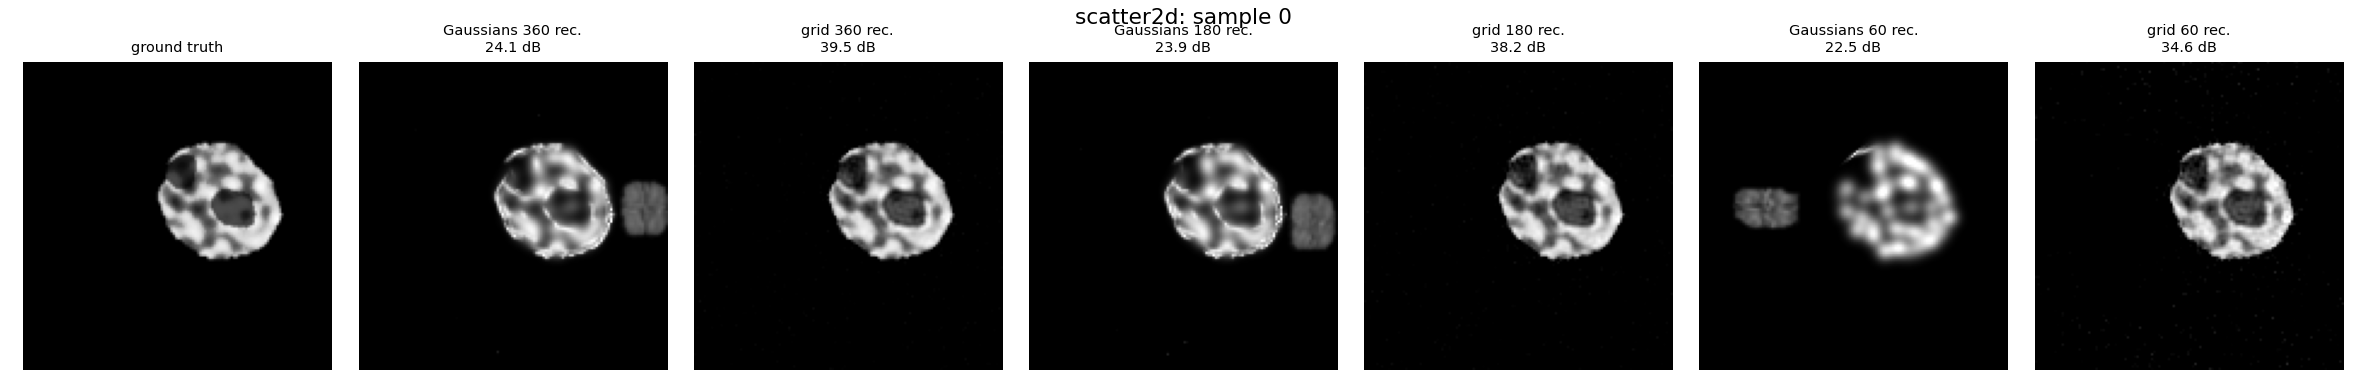
\includegraphics[width=\linewidth]{scatter2d_ghost.png}\\[2pt]
  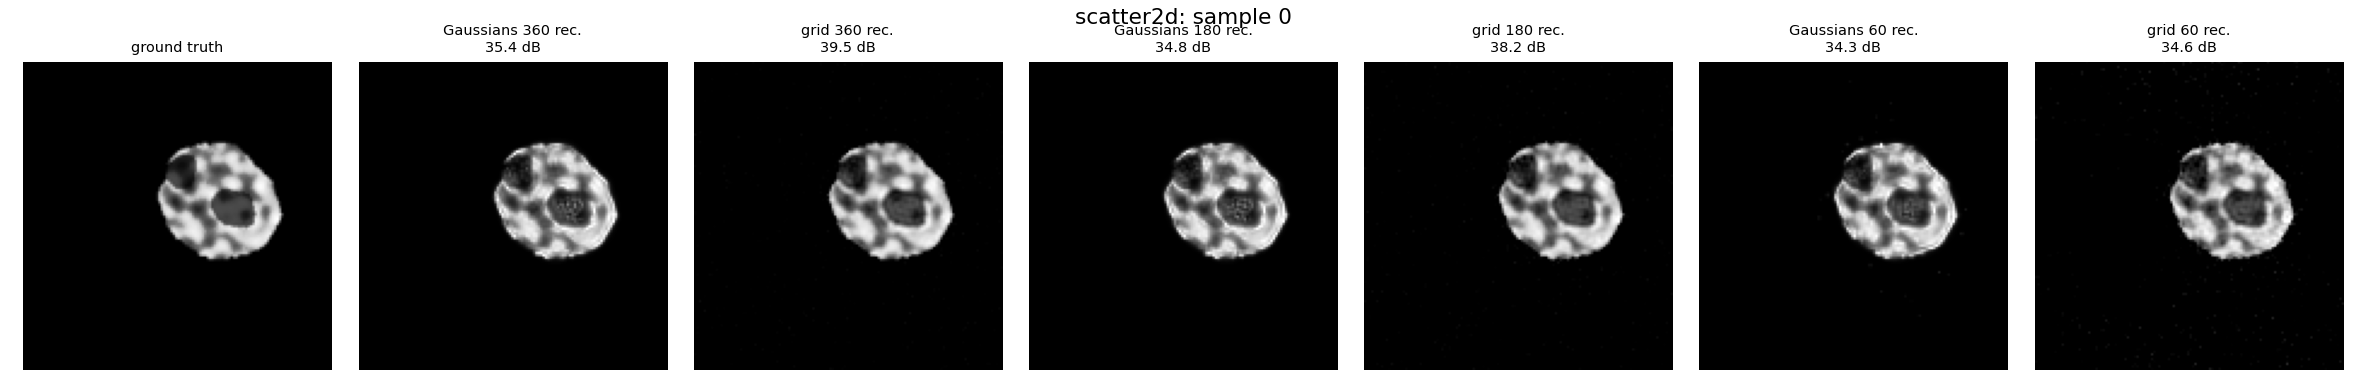
\includegraphics[width=\linewidth]{scatter2d_sparsity.png}
  \caption{Cell 0. Top: aggressive densification without regularisation produces a ghost copy beside the cell.
  Bottom: with the sparsity term ($\lambda=0.3$) the ghost is gone. Columns: ground truth, then Gaussian and pixel
  reconstructions at 360, 180 and 60 receivers.}
  \label{fig:ghost}
\end{figure}

\section{3D inverse scattering}
\label{sec:s3d}
On synthetic nuclei (Table~\ref{tab:s3d}, Figure~\ref{fig:s3d}) Gaussians are almost unaffected by the number of
receivers (40.6--40.9\,dB), while the voxel grid degrades from 44.1 to 37.3\,dB and becomes speckled. With 60
receivers Gaussians are better on all three volumes (+3.6\,dB on average) and have higher SSIM at every receiver
count.

The real CytoPacq nuclei from BBBC024 reverse this picture. The voxel grid reaches 35--42\,dB, while Gaussians stay at
27--28\,dB regardless of the number of receivers or the sparsity term. Figure~\ref{fig:s3d_bbbc} shows the reason: the
BBBC024 volumes are binary masks with sharp nucleus boundaries, and a sum of smooth Gaussians reproduces each
nucleus with a soft edge and a faint bright rim. The error is concentrated at the boundaries and is a
representation limit (the PSNR does not change with the receiver count), not a measurement limit. In SSIM, which is
less sensitive to edge error, Gaussians with sparsity (0.955) still beat the unregularised voxel grid (0.936) at 60
receivers, but not the voxel grid with the same sparsity (0.971). Together with the synthetic result this gives a
clear rule: Gaussians help when the object is smooth, and hurt when it is piecewise constant with sharp edges.

\begin{table}[h]
  \centering
  \caption{3D inverse scattering, $32\times128\times128$ volumes (PSNR dB / SSIM, mean of 3 volumes).}
  \label{tab:s3d}
  \resizebox{\linewidth}{!}{%
  \begin{tabular}{llccc}
    \toprule
    Volumes & Method & 360 receivers & 180 receivers & 60 receivers \\
    \midrule
    \multirow{2}{*}{Synthetic nuclei} & Gaussians & 40.8 / \textbf{0.994} & 40.6 / \textbf{0.994} & \textbf{40.9 / 0.988} \\
                                      & Voxel grid & \textbf{44.1} / 0.987 & \textbf{41.5} / 0.977 & 37.3 / 0.932 \\
    \midrule
    \multirow{4}{*}{BBBC024 (CytoPacq)} & Gaussians & 27.9 / 0.967 & 27.6 / 0.965 & 27.0 / 0.943 \\
                                         & Voxel grid & \textbf{41.8} / 0.989 & \textbf{40.3} / 0.980 & \textbf{35.3} / 0.936 \\
                                         & Gaussians + sparsity, $\lambda=0.3$ & 28.4 / 0.974 & 28.4 / 0.974 & 27.4 / 0.955 \\
                                         & Voxel grid + sparsity, $\lambda=0.3$ & 38.5 / \textbf{0.996} & 38.0 / \textbf{0.995} & 34.4 / \textbf{0.971} \\
    \bottomrule
  \end{tabular}}
\end{table}

\begin{figure}[h]
  \centering
  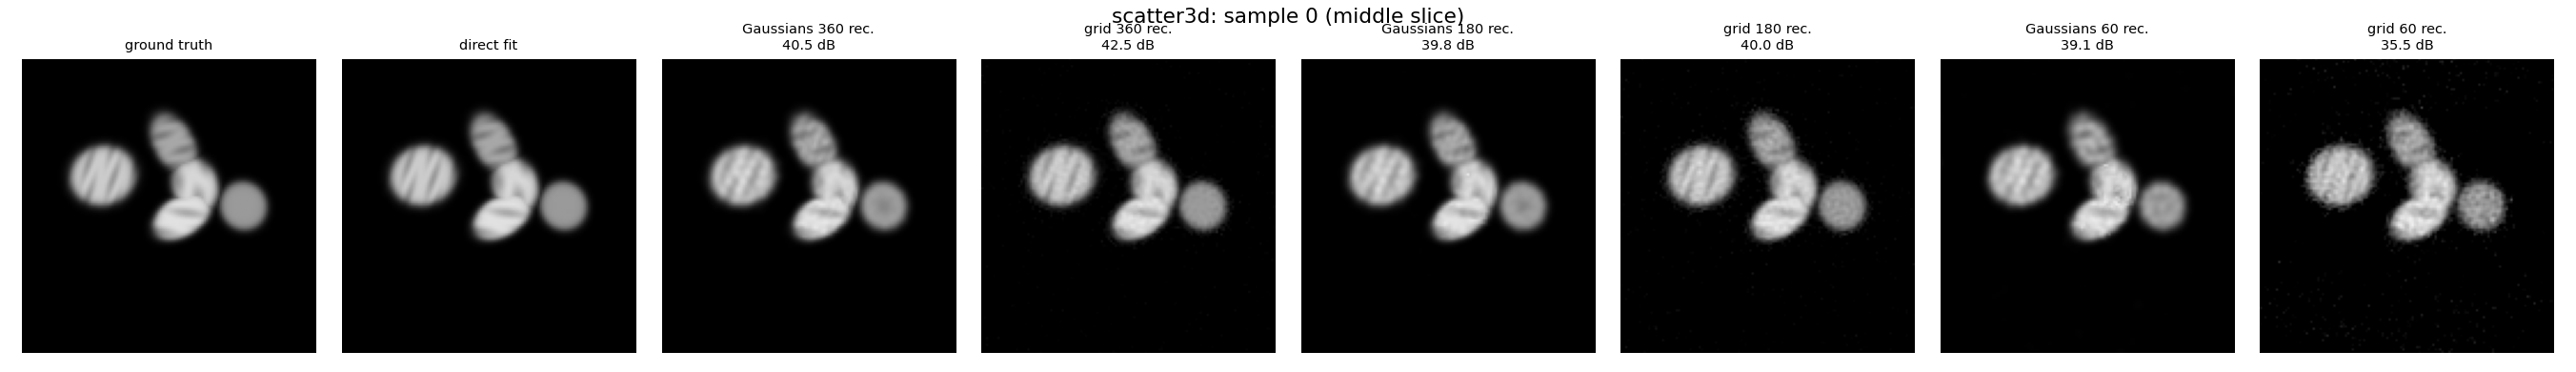
\includegraphics[width=\linewidth]{scatter3d_first.png}
  \caption{Middle slice of synthetic volume 0: ground truth, direct fit, then Gaussian and voxel reconstructions at
  360, 180 and 60 receivers.}
  \label{fig:s3d}
\end{figure}

\begin{figure}[h]
  \centering
  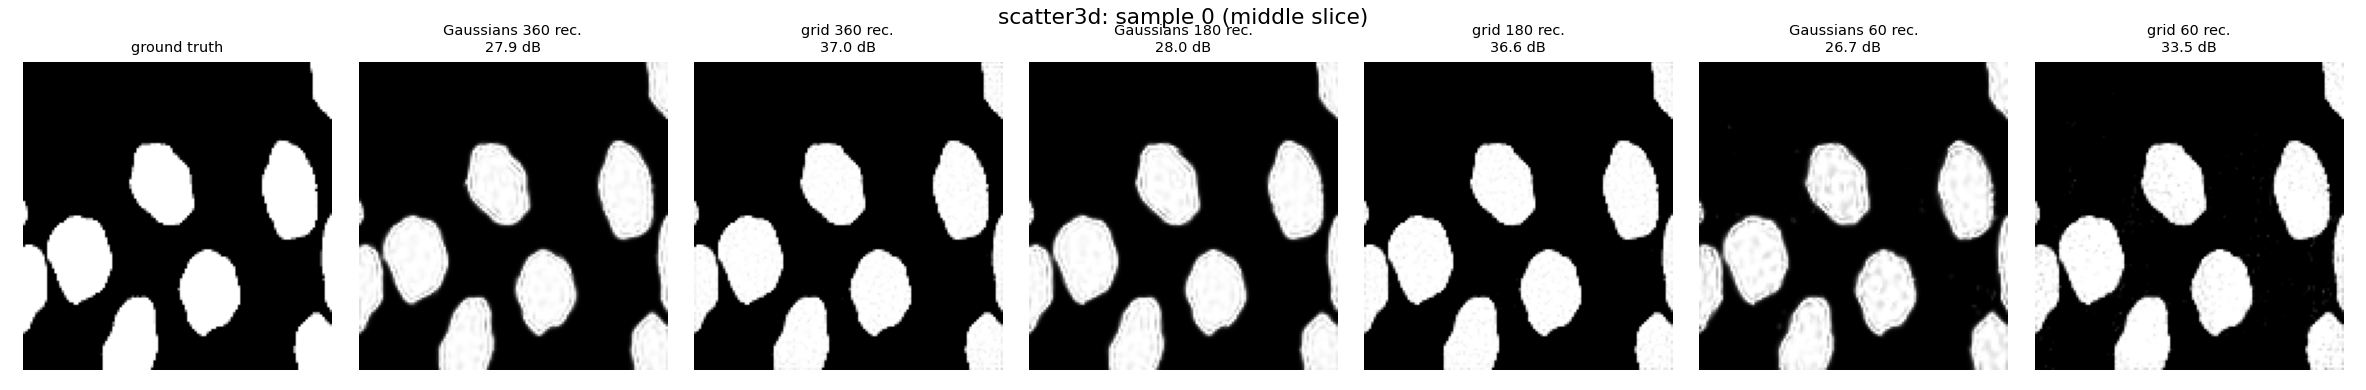
\includegraphics[width=\linewidth]{scatter3d_bbbc024.png}
  \caption{Middle slice of BBBC024 volume 0 (sparsity $\lambda=0.3$): ground truth, then Gaussian and voxel
  reconstructions at 360, 180 and 60 receivers. Gaussians soften the sharp nucleus boundaries and leave a faint rim.}
  \label{fig:s3d_bbbc}
\end{figure}

\section{4D Gaussians for Navier--Stokes}
Table~\ref{tab:ns} reports PSNR on held-out frames, with observed-frame PSNR in brackets. Static Gaussians reach only
about 17\,dB: the flow changes too much over 21 frames for one fixed field. A deformation network adds about 10\,dB.
Without regularisation, Mamba fits the observed frames much better than the MLP (36.1 vs.\ 30.3\,dB with full
observations), but on held-out frames the two are within 0.3\,dB: Mamba's extra capacity is spent memorising
observed times.

The final runs add the temporal smoothness term ($\lambda_T=1$). With 10\% of pixels observed, Mamba now generalises
clearly better than the MLP: 25.4 vs.\ 23.0\,dB on held-out frames, better on each of the three sequences
(+2.2, +2.0 and +2.9\,dB), and 2.3\,dB better than unregularised Mamba. The MLP is unchanged by the term, and the MLP
reconstructions show streak artefacts where data are sparse (Figure~\ref{fig:ns_smooth}). With full observations
all deformation models are within about 1\,dB (MLP 27.4, Mamba 27.2\,dB). The bidirectional Mamba fits observed frames
best but does not improve held-out frames (25.1 and 26.4\,dB) and doubles the training time. Mamba is about nine
times slower than the MLP (28 vs.\ 3\,min per sequence) because of its sequential pure-PyTorch scan.

\begin{table}[h]
  \centering
  \caption{4D Navier--Stokes, PSNR (dB) on held-out frames; observed-frame PSNR in brackets (mean of 3 sequences).
  ``+ smooth'' = temporal smoothness $\lambda_T=1$ (final runs).}
  \label{tab:ns}
  \resizebox{\linewidth}{!}{%
  \begin{tabular}{lcccc}
    \toprule
    Observed pixels & Static & MLP (4DGS-style) & Mamba & Bidirectional Mamba \\
    \midrule
    100\% & 17.0 (16.8) & 27.6 (30.3) & \textbf{27.9} (36.1) & -- \\
    100\% + smooth & -- & 27.4 (30.6) & 27.2 (35.2) & 26.4 (\textbf{36.5}) \\
    10\%  & 16.0 (15.9) & 23.2 (24.0) & 23.1 (27.7) & -- \\
    10\% + smooth & -- & 23.0 (24.1) & \textbf{25.4} (28.9) & 25.1 (\textbf{29.6}) \\
    \midrule
    Training time per sequence & 3\,min & 3\,min & 15--28\,min & 52\,min \\
    \bottomrule
  \end{tabular}}
\end{table}

\begin{figure}[h]
  \centering
  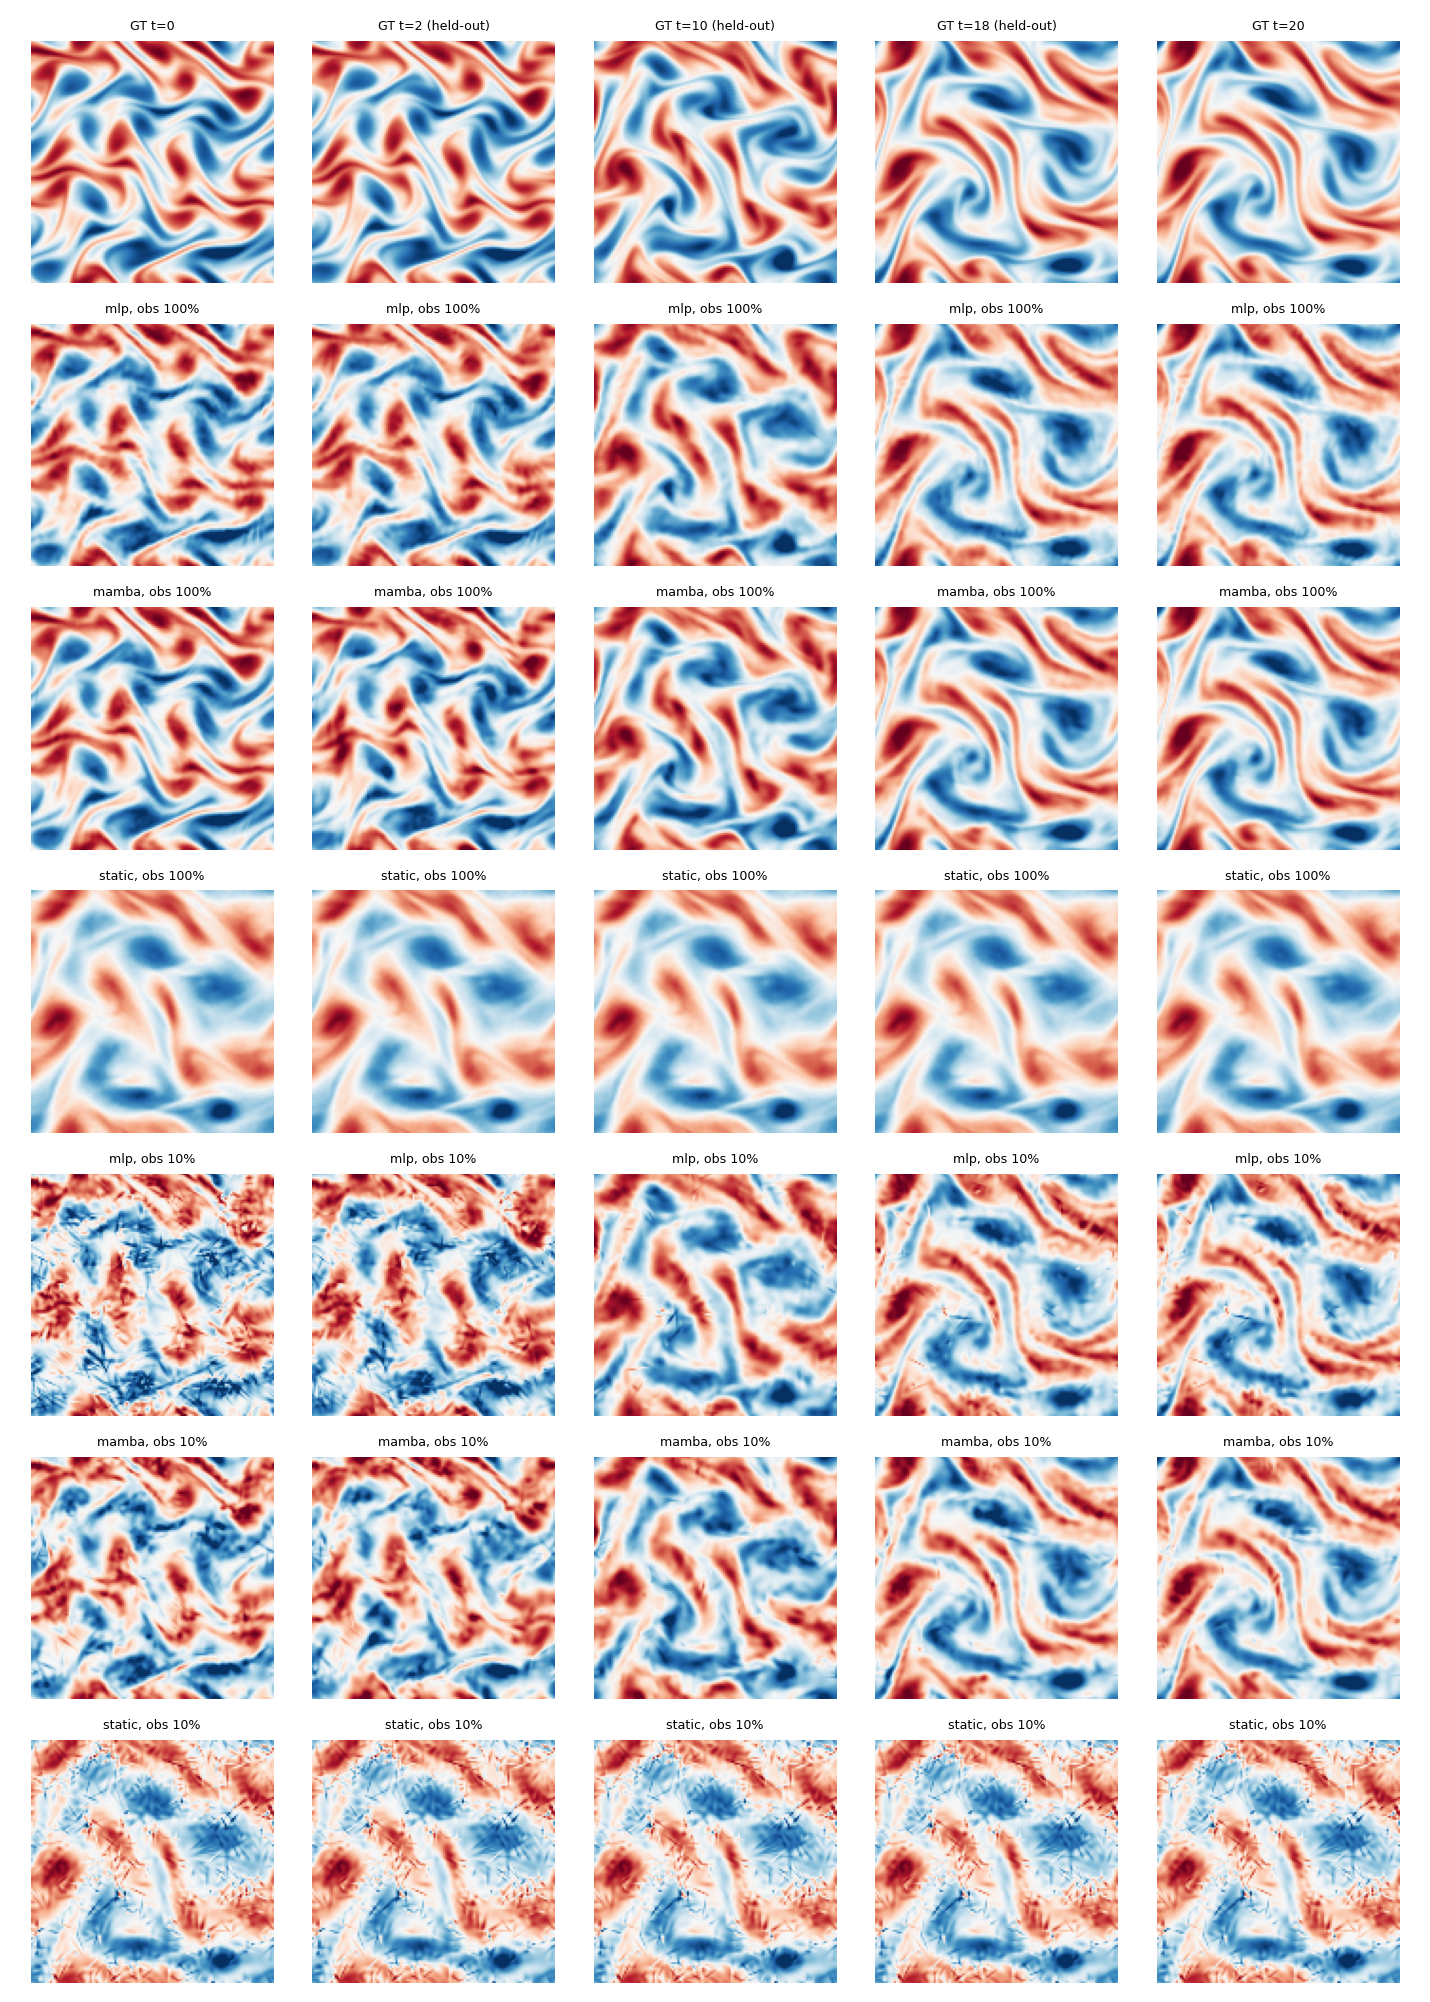
\includegraphics[width=0.85\linewidth]{ns4d_first.png}
  \caption{Initial runs: vorticity of sequence 0 at five times (held-out frames marked). Rows: ground truth, then
  MLP, Mamba and static models with 100\% and 10\% of pixels observed.}
  \label{fig:ns}
\end{figure}

\begin{figure}[h]
  \centering
  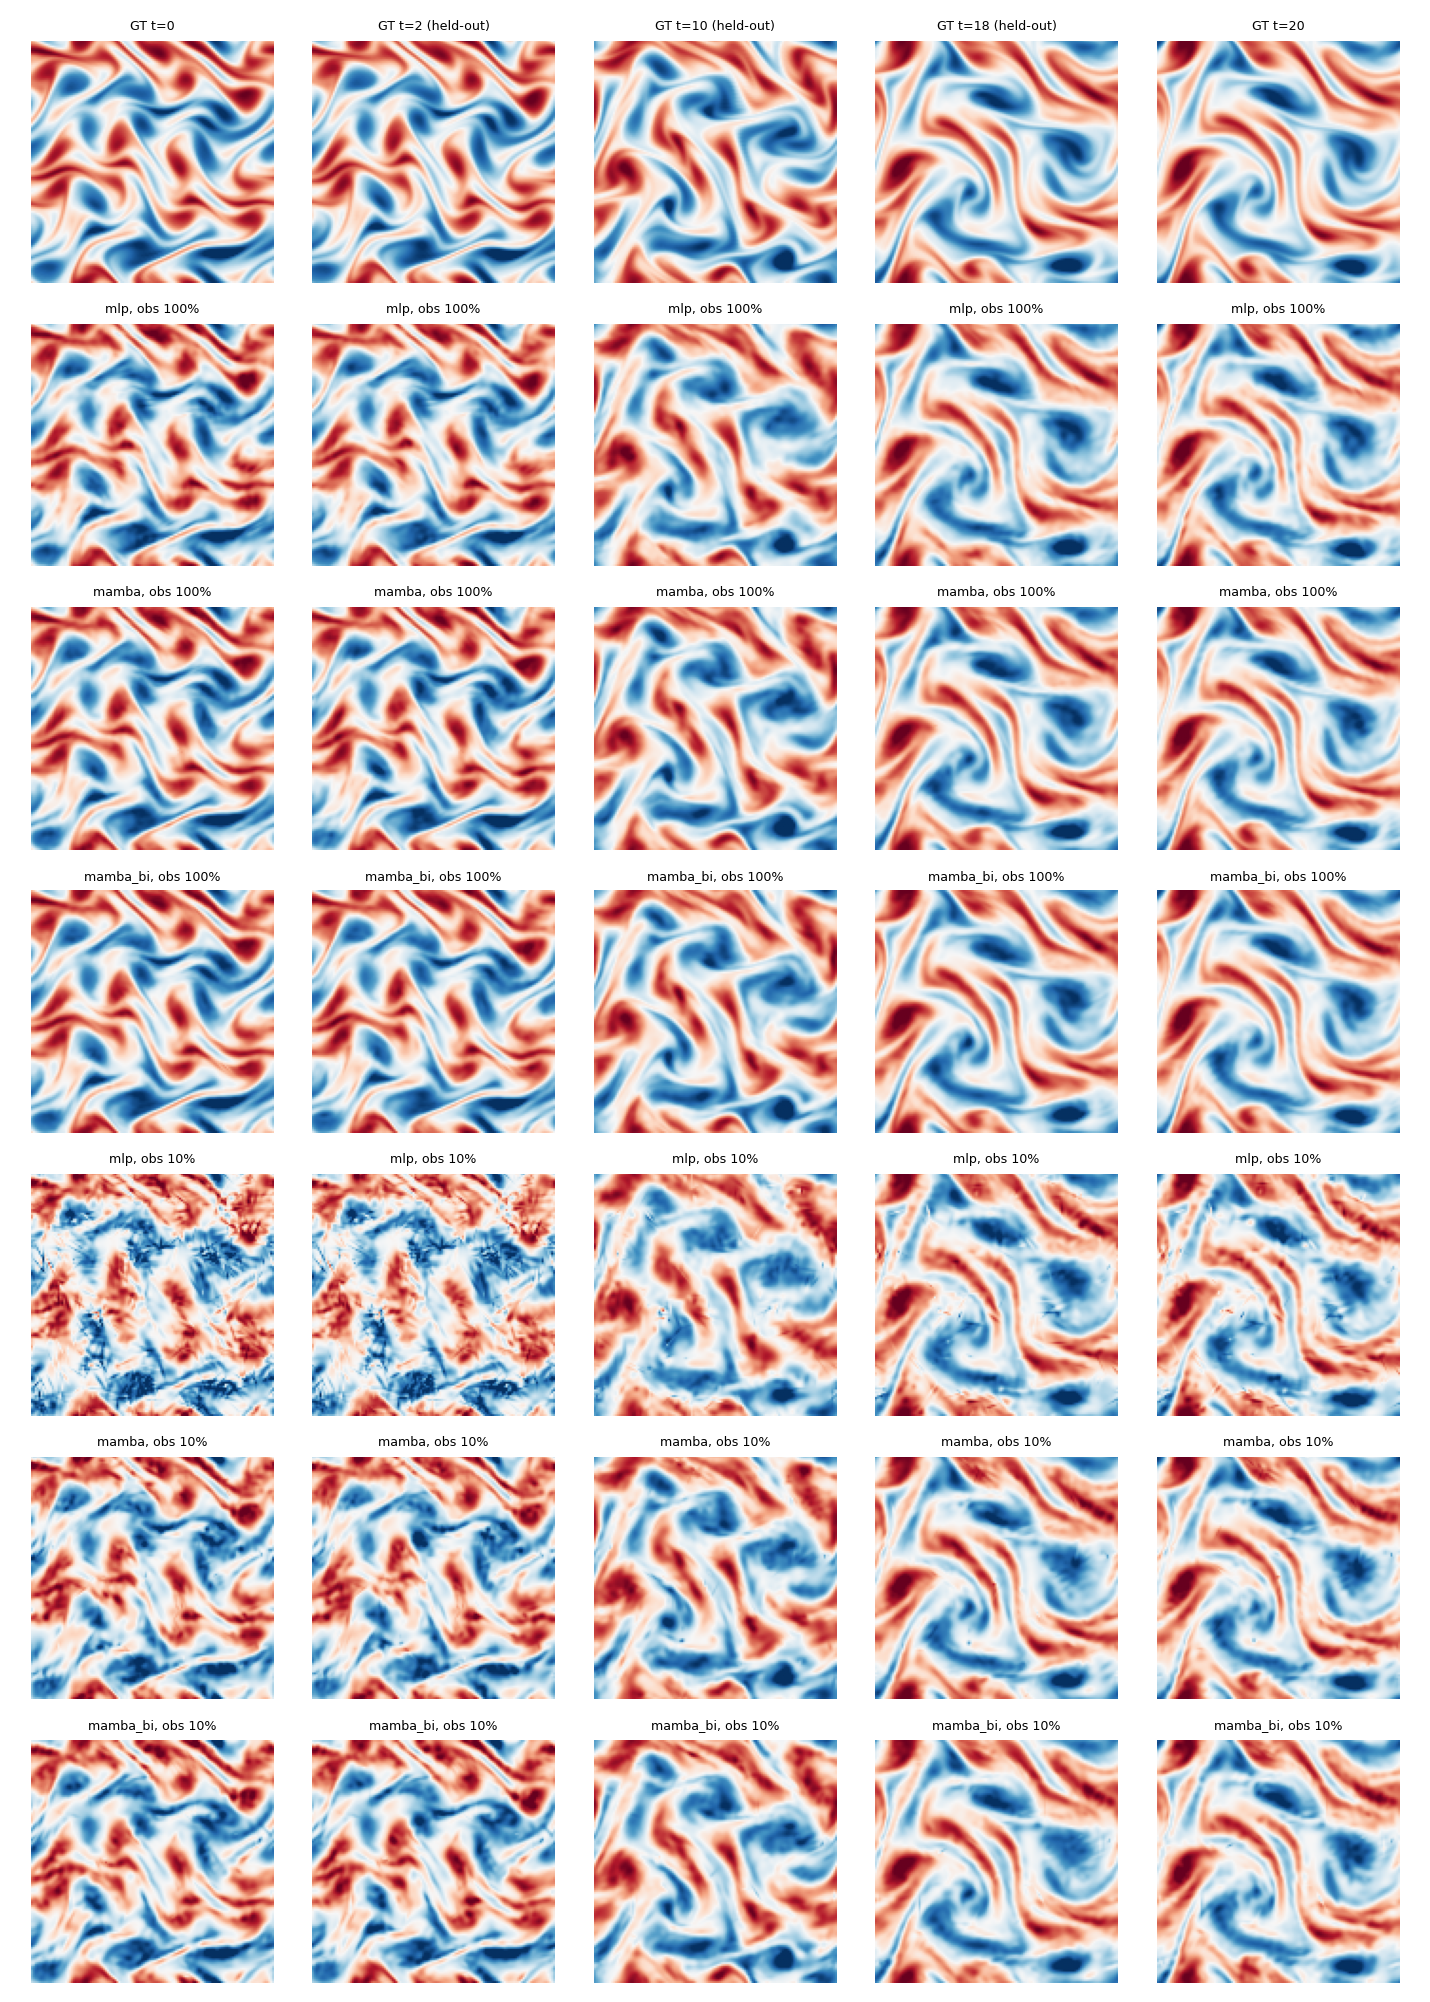
\includegraphics[width=0.75\linewidth]{ns4d_smooth.png}
  \caption{Final runs with temporal smoothness: ground truth, then MLP, Mamba and bidirectional Mamba with 100\% and
  10\% of pixels observed. With 10\% observations the MLP shows streaks; Mamba stays coherent.}
  \label{fig:ns_smooth}
\end{figure}

\section{Answers to the research questions}
\begin{description}
  \item[RQ1] Partly. On smooth 3D volumes Gaussians are more robust than voxels to scarce measurements (+3.6\,dB at 60
  receivers). On real, sharp-edged BBBC024 nuclei and on textured 2D cells the grid is better in PSNR; a grid with
  the same sparsity prior also matches or beats Gaussians in SSIM. The benefit depends on the object matching the
  smooth Gaussian prior.
  \item[RQ2] Adaptive densification can populate the operator's null space with ghost structures; a sparsity term on
  total intensity prevents them and is required for Gaussians.
  \item[RQ3] Yes: canonical Gaussians plus a deformation network reconstruct the flow at held-out times, about 10\,dB
  better than static Gaussians, from full or 10\% observations.
  \item[RQ4] Yes, when observations are sparse and the model is regularised in time: Mamba with temporal smoothness
  beats the MLP by 2.4\,dB on held-out frames with 10\% observations. With full observations there is no gain, and the
  bidirectional variant adds cost without benefit.
\end{description}

\chapter{Discussion, Limitations and Plan for Thesis II}
\label{ch:conclusion}

\section{Discussion}
Replacing the camera model of Gaussian splatting with a physics operator works: the same representation, optimiser and
density control recover cells from scattered fields and moving vorticity from sparse samples. The representation acts
as a prior that is helpful when the object matches it (smooth nuclei, scarce data) and neutral or harmful when it does
not (fine texture, abundant data). The most instructive finding is the ghost failure mode: adaptivity, the main
strength of Gaussian splatting with cameras, becomes a liability when the measurements are blind to part of the
domain, and must be balanced by an explicit prior. The final runs add a second lesson: a Gaussian sum is unbounded, and on physical quantities with a known range
this matters more than the shape of the kernel. Unbounded Gaussians lost to a clipped grid almost everywhere;
the bounded density $1-e^{-f}$, the same saturation as opacity in 3DGS, turned the true 3D results into a consistent
win with nine times fewer parameters, while sharper kernels did not help. For dynamics, the deformation model matters far more than the choice of network;
a sequence model pays off only once regularised in time, and then mainly when observations are sparse.

\section{Limitations}
\begin{itemize}
  \item The true 3D model is linear (first Born approximation); multiple scattering is not modelled, and 3D results
  use three volumes.
  \item Results use three to five samples per setting; differences of a few tenths of a dB are not yet significant.
  \item The 4D problem reconstructs a field from observations of itself; InverseBench's harder task of recovering the
  initial condition through the solver is not addressed.
  \item No learned prior is used, and no comparison with InverseBench's diffusion methods is made (by design for
  Thesis I).
  \item Hyper-parameters (sparsity weight, Gaussian budget, window size, smoothness weight) were tuned on few samples.
  \item Under better-conditioned measurements (slice-wise 3D, 2D with many receivers) bounded Gaussians remain
  slightly below a regularised grid.
\end{itemize}

\section{Plan for Thesis II}
\begin{enumerate}
  \item Multiple scattering in 3D, and better optimisation of Gaussians under the true 3D model (initialisation
  from a back-projection or grid solution, bounded densities).
  \item Systematic evaluation on the full InverseBench test sets with confidence intervals, and comparison with the
  benchmark's diffusion-prior methods.
  \item Physics-aware density control (densify only within the support indicated by the data; null-space-aware
  regularisers) instead of a global sparsity term.
  \item Bounded Gaussians on the full test sets with confidence intervals, and learned or adaptive saturation for
  quantities without a fixed range.
  \item Motion models: hardware-efficient Mamba (parallel scan), tuning of the smoothness weight, and advection-informed
  deformation that uses the velocity field implied by the vorticity.
  \item The Navier--Stokes initial-value inverse problem through a differentiable solver.
  \item Connection to the original direction of this work: attaching semantic features to physical Gaussians, in the
  spirit of LangSplat~\citep{qin2024langsplat} and 4D LangSplat~\citep{li2025langsplat4d}.
\end{enumerate}

\section{Conclusion}
This Thesis I establishes a working, reproducible proof of concept for 3D and 4D Gaussian representations in two
scientific inverse problems, identifies when they help and how they fail, and defines the experiments that Thesis II
will scale up.


\bibliographystyle{plainnat}
\bibliography{references}

\appendix
\chapter{Reproducibility}
\label{app:repro}

The code, configurations and results are in the thesis repository (\texttt{src/thesis\_gs} package, \texttt{bin/}
scripts, \texttt{configs/}, \texttt{notebooks/}, \texttt{results/}, \texttt{tests/}). InverseBench and its test data are
downloaded automatically; BBBC024 is downloaded by the Kaggle notebook.

{\small
\begin{verbatim}
# install, smoke test, 2D run, final runs, unit tests
pip install -r requirements.txt
python bin/thesis-gs --task all --quick --out outputs/smoke
python bin/thesis-gs --task scatter2d --l1 0.3 --out outputs/s2d
python bin/run_experiments.py configs/final_part_a.json \
       --out outputs/final_a --volumes /path/to/BBBC024
python bin/run_experiments.py configs/final_part_b.json \
       --out outputs/final_b
pytest -q
\end{verbatim}
}

Every run writes \texttt{run\_config.json} with its exact settings, \texttt{results.csv} with per-sample metrics,
\texttt{summary.csv} with means, and \texttt{reconstructions.png}.


\end{document}
